\documentclass[tikz,border=2pt]{standalone}
\usepackage{amsmath,amssymb}
\usepackage{tikz}

\begin{document}
% The minimum spanning tree of the example network: edges B-C, A-C, D-E, E-F, B-D, total 13,
% the cheapest way to connect all six vertices.
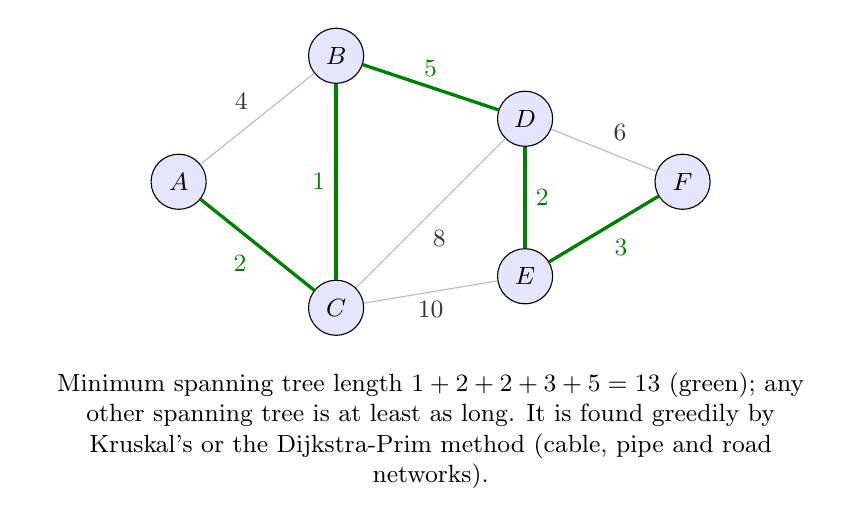
\begin{tikzpicture}[every node/.style={font=\small}, v/.style={draw, circle, fill=blue!10, minimum size=7mm, inner sep=0pt}]
	\node[v] (A) at (0,0) {$A$};
	\node[v] (B) at (2,1.6) {$B$};
	\node[v] (C) at (2,-1.6) {$C$};
	\node[v] (D) at (4.4,0.8) {$D$};
	\node[v] (E) at (4.4,-1.2) {$E$};
	\node[v] (F) at (6.4,0) {$F$};
	\draw[gray!55] (A) -- (B) node[midway, above left, text=gray!40!black] {$4$};
	\draw[gray!55] (C) -- (D) node[pos=0.45, below right, text=gray!40!black] {$8$};
	\draw[gray!55] (C) -- (E) node[midway, below, text=gray!40!black] {$10$};
	\draw[gray!55] (D) -- (F) node[midway, above right, text=gray!40!black] {$6$};
	\draw[green!50!black, very thick] (A) -- (C) node[midway, below left] {$2$};
	\draw[green!50!black, very thick] (B) -- (C) node[midway, left] {$1$};
	\draw[green!50!black, very thick] (B) -- (D) node[midway, above] {$5$};
	\draw[green!50!black, very thick] (D) -- (E) node[midway, right] {$2$};
	\draw[green!50!black, very thick] (E) -- (F) node[midway, below right] {$3$};
	\node[anchor=north, align=flush center, text width=10cm] at (3.2,-2.3) {Minimum spanning tree length $1+2+2+3+5=13$ (green); any other spanning tree is at least as long. It is found greedily by Kruskal's or the Dijkstra-Prim method (cable, pipe and road networks).};
\end{tikzpicture}
\end{document}
